\documentclass[11pt]{article}
\usepackage[utf8]{inputenc}
\usepackage[T1]{fontenc}
\usepackage[francais]{babel}
\usepackage[francais]{layout}
\usepackage{hyperref}
\selectlanguage{french}

% NE PAS CHANGER !!
\ifx \public \undefined \def\public{etudiants} \fi
\usepackage[\public]{tps}
\usepackage{tikz}

% Numéro du TP
\newcommand{\numtd}{03}
% Titre du TP
\newcommand{\titretd}{Logic circuits and Bitwise operation}
\def\tup#1{\langle #1\rangle}
\begin{document}
	
	\entete{\numtd}{\titretd}


\subsection*{Exercises 1}
We want to display the hexadecimal value of a 4-bit number on a 7-segment display. The LEDs are lit with a logical ‘0’ (negative logic or active low). The inputs are active high (or in positive logic). 
\begin{enumerate}
    \item Complete the truth table for each output (a-g).
    \item Provide an expression based on minterm for each output.
    \item Draw the logic circuit of the output a. 
\end{enumerate}


\begin{center}
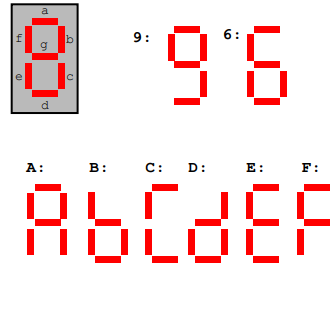
\includegraphics{7-segment.png}    
\end{center}



\subsection*{Exercises 2}
A binary decoder is a combinational logic circuit that converts binary information from the $n$ coded inputs to a maximum of $2^n$ unique outputs. You can see the truth table for the 3-to-3-line decode in the following: 

\begin{center}
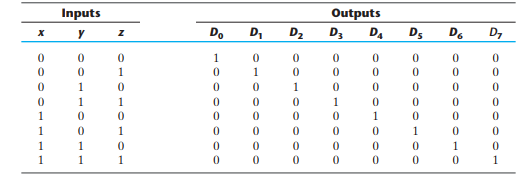
\includegraphics{Ex0.png}    
\end{center}

For each possible input combination, there are seven outputs that are equal to 0 and only one that is equal to 1. The output whose value is equal to 1 represents the minterm equivalent of the binary number currently available in the input lines. 

An application of decoder to construct a 4-to-1-line multiplexer:

\begin{center}
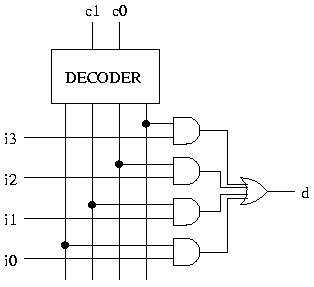
\includegraphics{Decoder.png}    
\end{center}


\begin{enumerate}
    \item Construct 5-to-32-line decoder with four 3-to-8-line decoder with enable and one 2-to-4-line decoder (Use the block diagrams).
    \item Draw the logic diagram of a 2-to-4-line decoder with only NOR gates. Include an enable input.
    \item Construct a 16-to-1-line multiplexer with two 8-to-1-line multiplexer and one 2-to-1-line multiplexer (Use the block diagrams). 
\end{enumerate}



\subsection*{Exercises 3}
Design a circuit (simplify your circuit) that verifies the logical operation of a XOR gate. f = '1' (LED ON) if the XOR gate does NOT work properly. Assumption: when the XOR gate is not working, it
generates 1's instead of 0's and vice versa.

\begin{center}
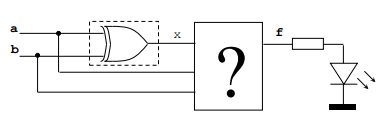
\includegraphics{Ex1.png}    
\end{center}



\subsection*{Exercises 4}
Design a logic circuit (simplify your circuit) that opens a lock (f = ‘1’) whenever one presses the correct number on each numpad. We encode each decimal number on the numpad using BCD encoding. We expect that each group of 4 bits be in the range from 0000 to 1001, the values from 1010 to 1111 are assumed not to occur.

\begin{center}
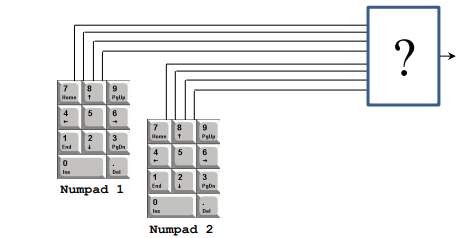
\includegraphics{Ex2.png}    
\end{center}


\subsection*{Exercises 5}
A  sequential circuit is a type of logic circuit whose output depends not only on the present value of its input signals but on the sequence of past inputs. This is in contrast to combinational logic, whose output is a function of only the present input. That is, sequential logic has state (memory) while combinational logic does not. The basic memory element in sequential logic is the flip-flop. There are different flip-flops such as S-R, J-K, and D flip-flop. 



\bigskip

The function table and sequential circuit of the S-R flip-flop is as following: 

\begin{center}
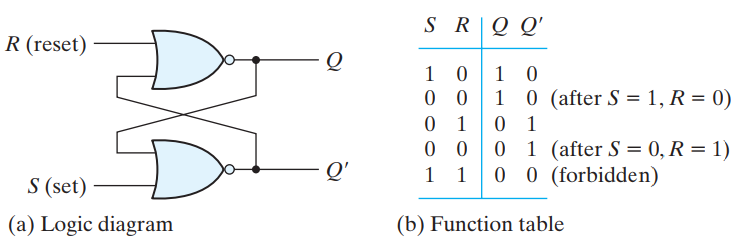
\includegraphics[width=120mm,scale=4]{SR.png}    
\end{center}


The D-type flip-flop is a modified S-R flip-flop with the addition of an inverter to prevent the S and R inputs from being at the same logic level.

\begin{itemize}
    \item Draw the function table and sequential circuit of D flip-flop.
\end{itemize}


\bigskip


The JK flip-flop augments the behavior of the SR flip-flop by interpreting the J = K = 1 condition as a "flip" or toggle command. One can constrcut the circuit diagram of a J-K flip-flop with a D flip-flop and gates using the following equation:
\begin{center}
    $D=JQ'+K'Q$
\end{center}

\begin{itemize}
    \item  Draw the circuit of the J-K flip-flop.
\end{itemize}

\bigskip


One can also show the behavior of a flip-flop using the characteristic table. A characteristic table defines the logical properties of a flip-flop by describing its operation in tabular form. The characteristic tables of S-R and D flip-flop are presented as following. They define the next state as a function of the inputs and the present state. Q(t) refers to the present state,and Q(t + 1) is the next state.

\begin{center}
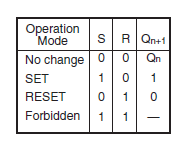
\includegraphics[width=40mm,scale=0.5]{S-R-char.png}\quad
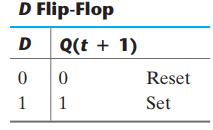
\includegraphics[width=40mm,scale=0.5]{D-cahr-table.png}
\end{center}


\begin{itemize}
    \item What is the characteristic table of the J-K flip-flop?
\end{itemize}



\subsection*{Exercises 6}

Show that a J-K flip-flop can be converted to a D flip-flop with an inverter between the J and K inputs.


A sequential circuit has two D flip-flops A and B, two inputs x and y, one output z. The flip-flop input equations and the circuit output are as follows: 
\begin{center}
    $D_A=x'y + xA$
    
    $D_B=x' B+xA$
    
    $z=B$
\end{center}

\begin{itemize}
    \item Draw the logical diagram of the circuit. 
    \item Tabulate the state table. 
\end{itemize}


\subsection*{Exercises 7}
Draw a sequential circuit with two J-K flip-flop A and B and two inputs x and E. If E$=0$, the circuit remains in the same state regardless of the value of x. When E$=1$ and x$=1$, the circuit goes through the state transition from 00 to 01 to 10 to 11 back to 00, and repeat. When E$=1$ and x$=0$, the circuit goes through the state transition from 00 to 10 to 01 back to 00, and repeat. 



\end{document}
